\documentclass{article}

\usepackage{graphicx}
\usepackage{indentfirst}
\usepackage[a4paper, total={6in, 8in}]{geometry}
\usepackage{hyperref}
\usepackage{fancyhdr}
\usepackage{xepersian}
\settextfont{XB Zar.ttf}
\setlatintextfont{Times New Roman.ttf}

\begin{document}


%title page%
\begin{titlepage}
	\begin{center}
		\vspace{0.2cm}
		
		
\includegraphics[width=0.4\textwidth]{sharif.png}\\
		\vspace{0.2cm}
		\textbf{ \Huge{آزمایش شماره 2}}\\
		\vspace{0.25cm}
		\textbf{ \Large{آز شبکه - دکتر بردیا صفایی}}
		\vspace{0.2cm}
		
		
		\large \textbf{دانشکده مهندسی کامپیوتر}\\\vspace{0.1cm}
		\large   دانشگاه صنعتی شریف\\\vspace{0.2cm}
		\large   ﻧﯿﻢ‌سال اول ۰۱-۰۲ \\\vspace{0.10cm}
		\large{ گروه 0:}\\
		\large{\href{mailto:mehrshad.mirmohammadi@gmail.com}{مهرشاد میرمحمدی - 98109634}}\\
		\large{\href{mailto:parhaamsaremi@gmail.com}{پرهام صارمی - 97101959}}\\
		\large{\href{mailto:mofayezi.m@gmail.com}{محمدرضا مفیضی - 98106059}}\\
	\end{center}
\end{titlepage}
%title page%

\newpage

%pages header
\pagestyle{fancy}
\fancyhf{}
\fancyfoot{}
\setlength{\headheight}{59pt}
\cfoot{\thepage}
\lhead{آزمایش شماره 2}
\rhead{
\includegraphics[width=0.1\textwidth]{sharif.png}\\
		دانشکده مهندسی کامپیوتر
}
\chead{آز شبکه - گروه ۰}
%pages header
\section{بخش اول}
با توجه به اینکه سایت sharif.edu از HTTPS استفاده می‌کرد از سایت old.sharif.edu استفاده شده است. زیر پس از capture کردن اطلاعات روی دامنه‌ی sharif.edu و فیلتر کردن آن خروجی‌ای مشاهده نشد. خروجی این عملیات را می‌توان در شکل \ref{fig:result} مشاهده کرد.
\begin{figure}[h!]
	\centering
	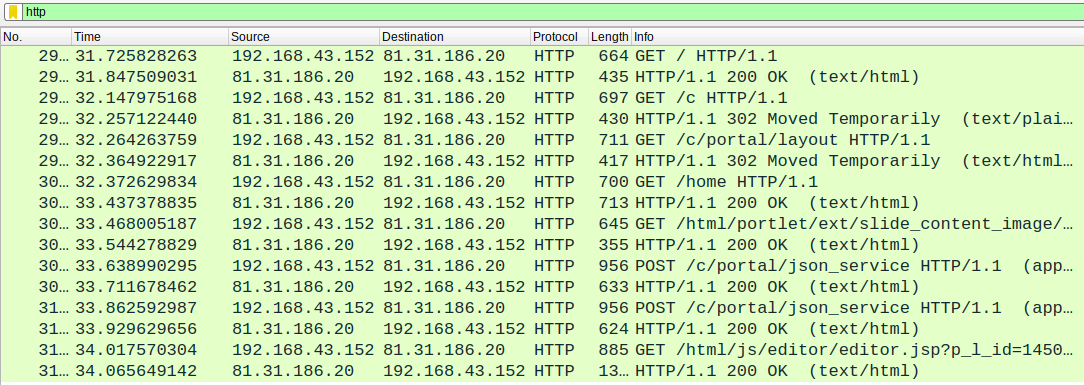
\includegraphics[width=0.9\textwidth]{src/result.png}
	\caption{
خروجی wireshark برای سایت old.sharif.edu	
}
	\label{fig:result}
\end{figure}

\subsection{سوال اول}
همانطور که در شکل \ref{fig:stat}مشاهده می‌شود بیشترین پروتوکل مورد استفاده TCP می‌باشد که ۳.۹۷ درصد از استفاده را به خود اختصاص داده است. با این حال مشاهده می‌شود که فقط ۱.۰ درصد از استفاده مربوط به داده‌های HTTP می‌باشد. علت این واقع باز بودن سایت‌ها و اپلیکیشن‌های دیگر در هنگام آزمایش بوده است. 
\begin{figure}[h!]
	\centering
	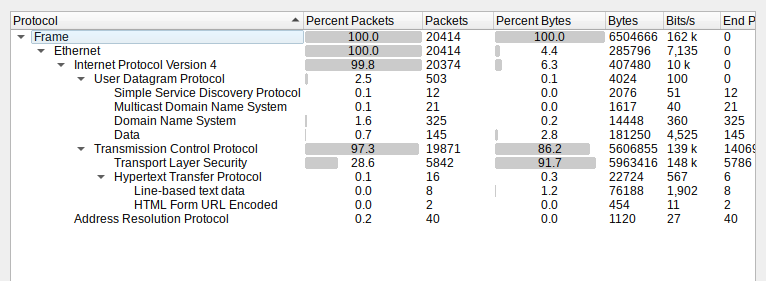
\includegraphics[width=0.9\textwidth]{src/stat.png}
	\caption{آمار‌های مشاهده شده در سوال ۱ آزمایش ۱ قبل از فیلتر کردن توسط http}
	\label{fig:stat}
\end{figure}

در  صورتی که ابتدا با HTTP بسته‌ها را فیلتر کنیم و پس از آن آمار را تماشا کنیم، متوجه می‌شویم که ۱۰۰ درصد بسته‌ها از نوع HTTP می‌باشند. برای دیدن نتایج می‌توانید به شکل \ref{fig:stat2} مراجعه کنید.
\begin{figure}[h!]
	\centering
	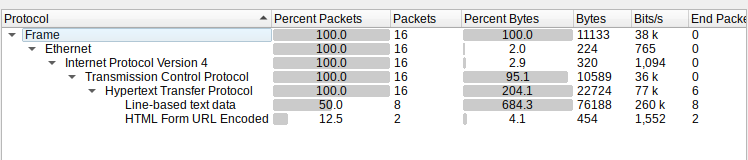
\includegraphics[width=0.9\textwidth]{src/stat2.png}
	\caption{آمار‌های مشاهده شده در سوال ۱ آزمایش ۱ پس از فیلتر کردن توسط http}
	\label{fig:stat2}
\end{figure}
\subsection{سوال دوم}
مطابق شکل \ref{fig:result} متوجه می‌شویم که زمان دریافت جواب حدودا برابر با ۱۲.۰ ثانیه می‌باشد. همچنین با توجه به شکل \ref{fig:tcpseq} می‌توان متوجه شد که 
\lr{seq number}
 برای اولین درخواست TCP برابر با \textbf{3614955439} بوده است. (برای دریافت این تنظیمات روی یک packet کلیک کرده و از زیرمنوی follow گزینه‌ی
  \lr{TCP Stream}
   زا انتخاب کردیم)
\begin{figure}[h!]
	\centering
	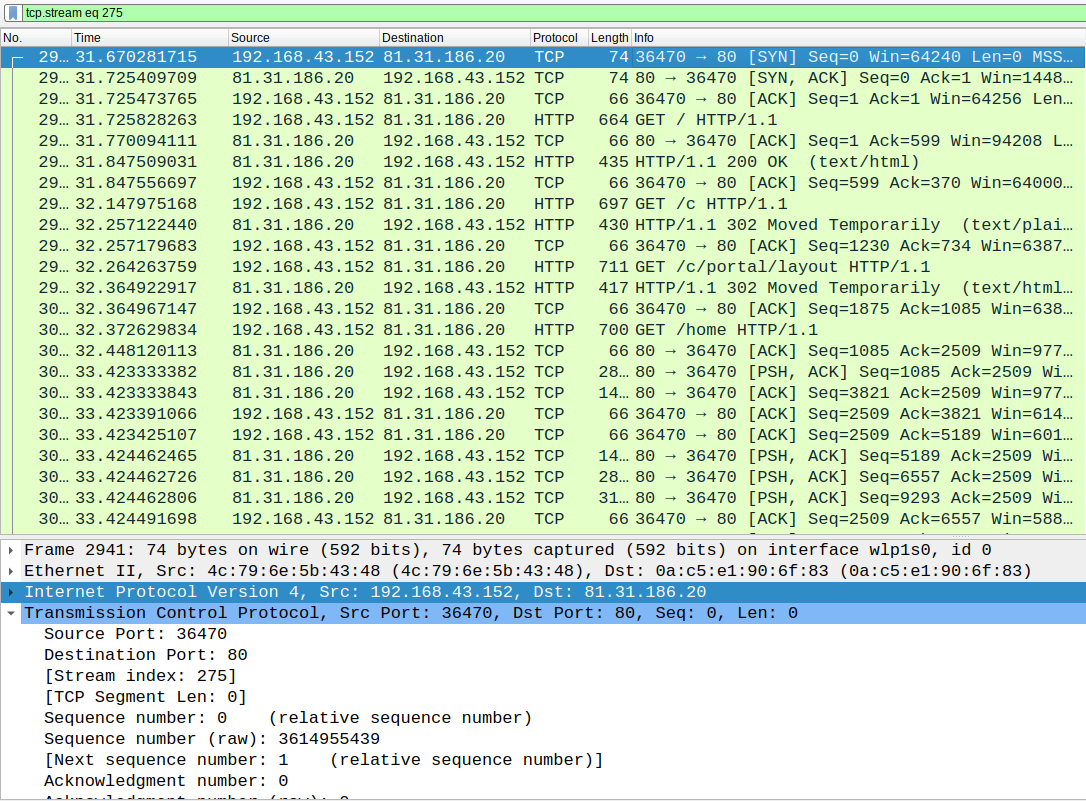
\includegraphics[width=0.9\textwidth]{src/tcpseq.png}
	\caption{
خروجی
 \lr{TCP Stream}
  که به ما این قابلیت را می‌دهد تا به صورت ریز خروجی‌ها را مشاهده کنیم.	
}
	\label{fig:tcpseq}
\end{figure}
\subsection{سوال سوم}
طبق شکل‌های \ref{fig:dnsreq} و \ref{fig:dnsresp} مشاهده می‌شود که هم درخواست و هم جواب هر دو از نوع A می‌باشند.
\begin{figure}[h!]
	\centering
	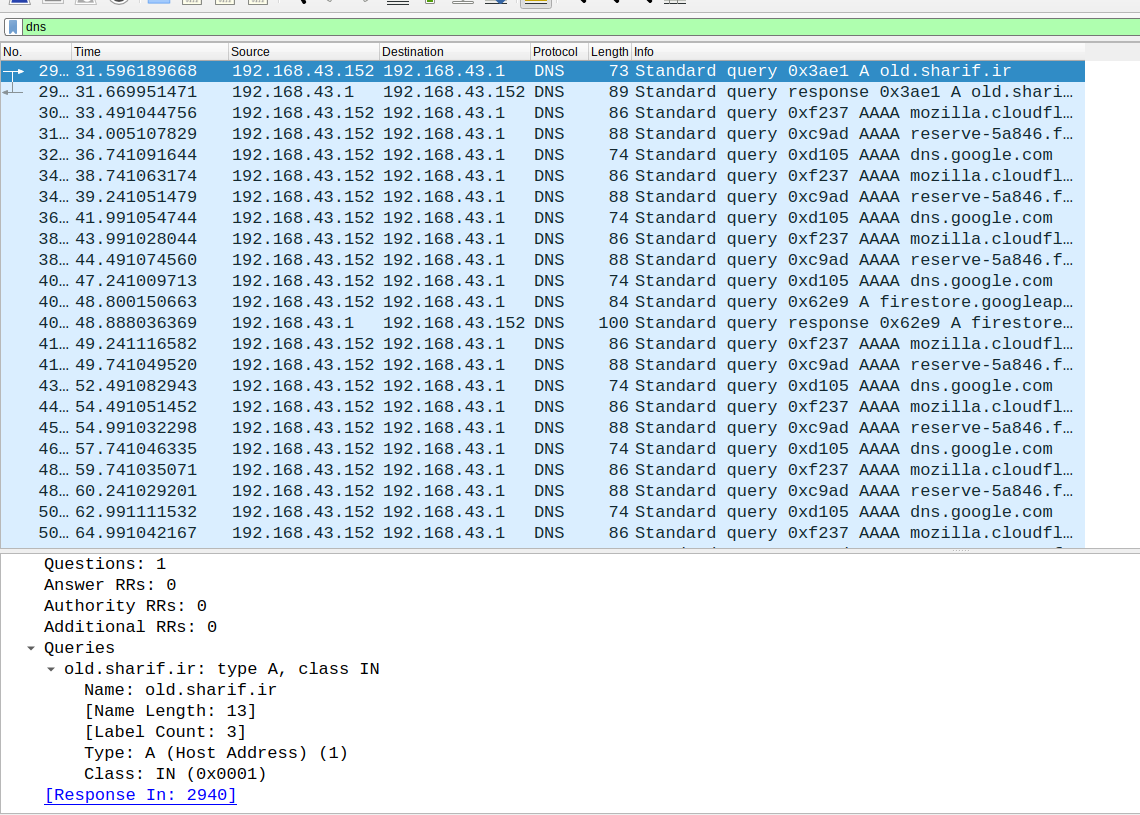
\includegraphics[width=0.9\textwidth]{src/dnsreq.png}
	\caption{
		درخواست DNS	
	}
	\label{fig:dnsreq}
\end{figure}
\begin{figure}[h!]
	\centering
	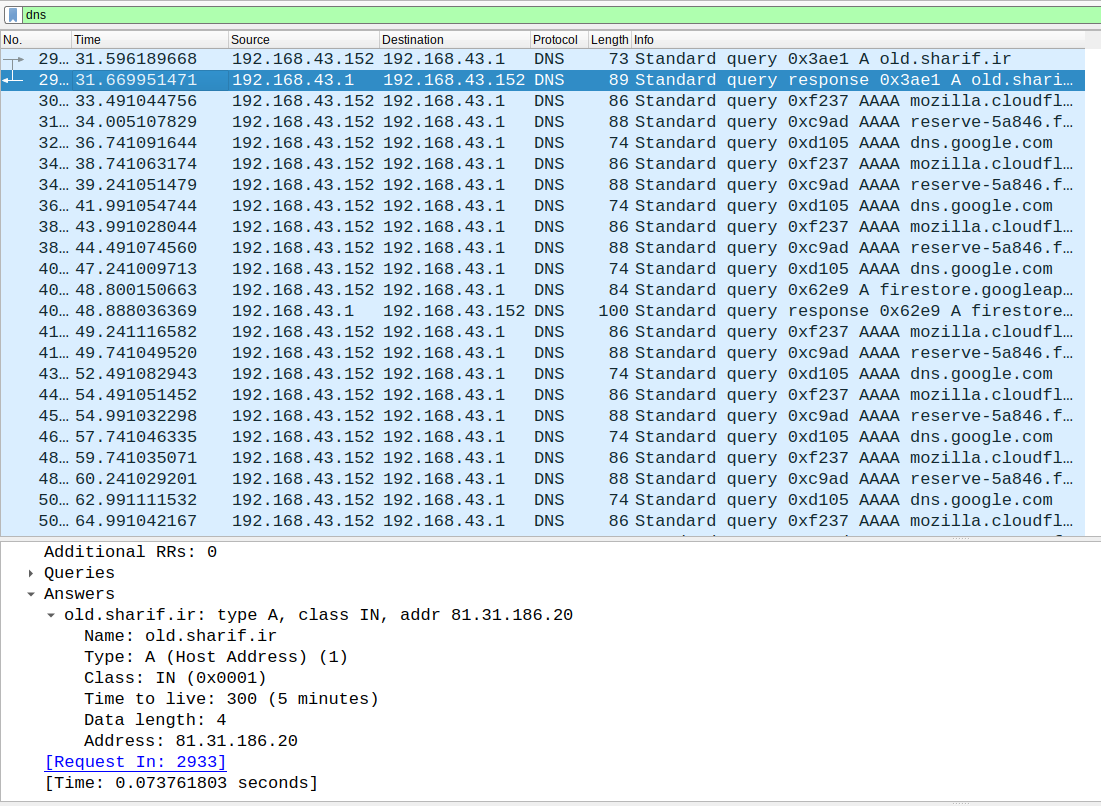
\includegraphics[width=0.9\textwidth]{src/dnsresp.png}
	\caption{
		جواب DNS	
	}
	\label{fig:dnsresp}
\end{figure}
\subsection{سوال چهارم}
در این قسمت متوجه شدیم که در خروجی‌های قسمت قبل عکسی وجود ندارد. علت این واقعه به این دلیل است که احتمالا مرورگر عکس‌ها را در دفعات قبلی باز کردن سایت cache کرده بود. بنابراین با استفاده از کلید Ctrl+F5 توانستیم cache را پاک کرده و عکس‌ها را از اول دریافت کنیم. سپس با استفاده از فیلتر image-jiff عکس‌های دریافت شده را فیلتر کردیم. عکس‌های دریافت شده در شکل \ref{fig:imgaes} دیده می‌شوند.
\begin{figure}[h!]
	\centering
	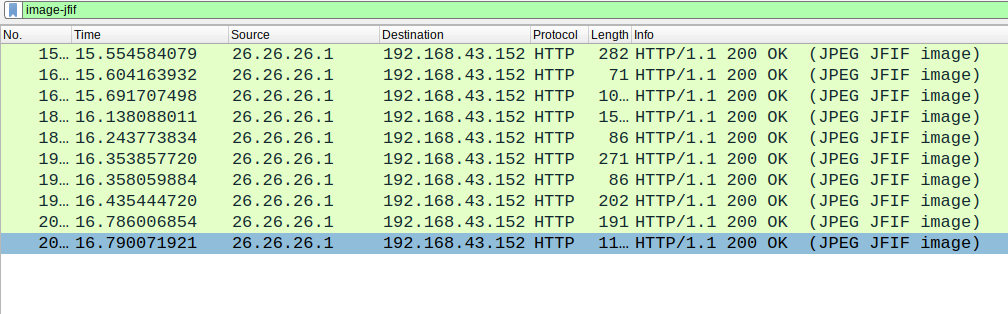
\includegraphics[width=0.9\textwidth]{src/image.png}
	\caption{
		عکس‌های دریافت شده
	}
	\label{fig:imgaes}
\end{figure}
با انتخاب یک عکس و انتخاب گزینه‌ی 
\lr{JPEG File Interchange Format} 
مانند شکل \ref{fig:imgstep} و زدن دکمه‌ی Ctrl+X می‌توان خروجی عکس را دریافت کرد. همچنین خروجی در شکل \ref{fig:extracted} دیده می‌شود.
\begin{figure}[h!]
	\centering
	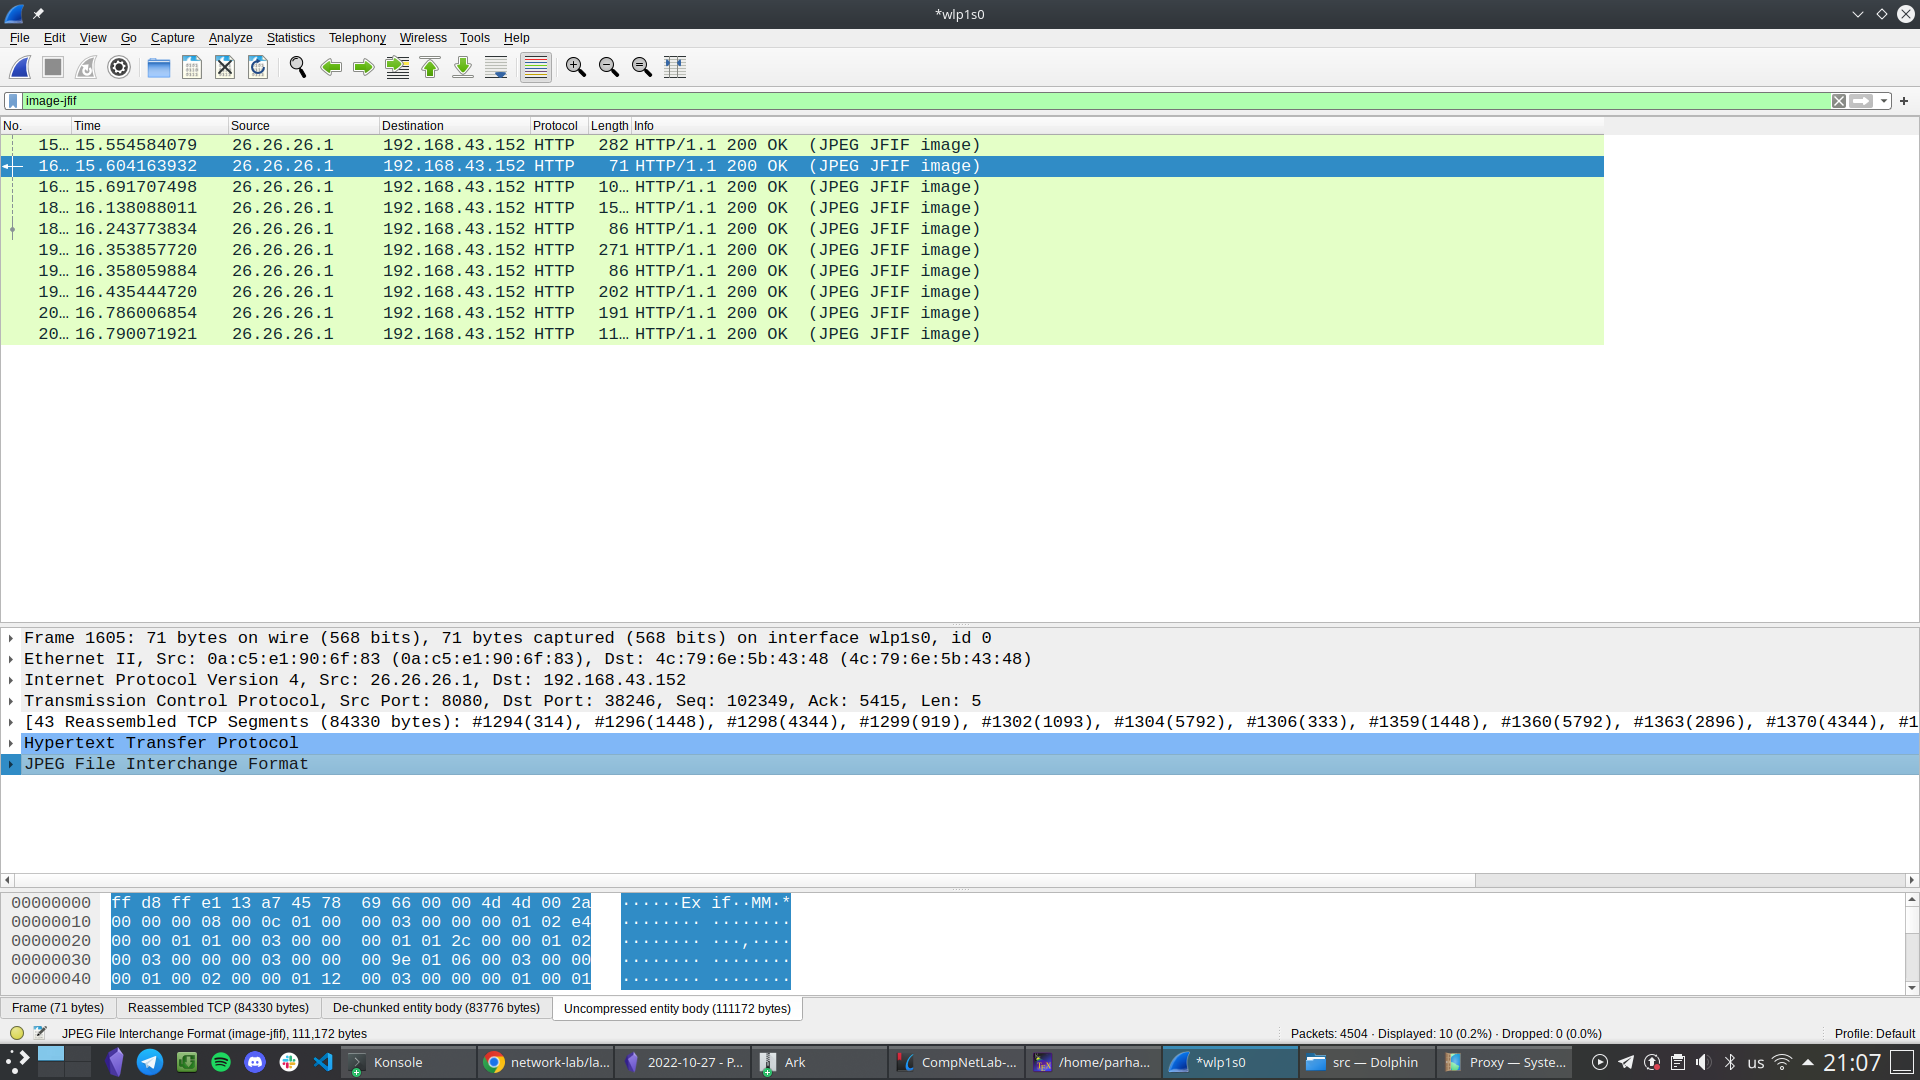
\includegraphics[width=0.9\textwidth]{src/imgstep.png}
	\caption{
		مراحل خروجی گرفتن عکس
	}
	\label{fig:imgstep}
\end{figure}
\begin{figure}[h!]
	\centering
	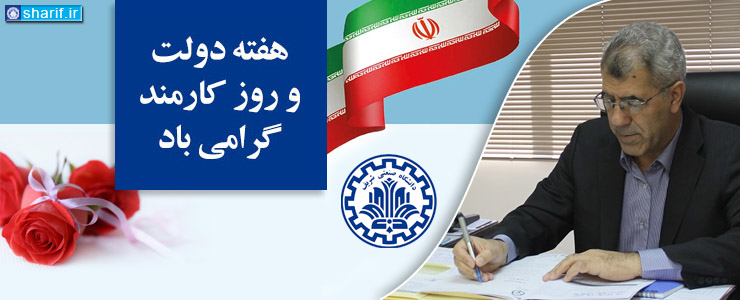
\includegraphics[width=0.9\textwidth]{src/extracted.png}
	\caption{
		عکس خروجی
	}
	\label{fig:extracted}
\end{figure}
\section{بخش دوم}
با استفاده از دستور 
\lr{telnet telehack.com} 
در ترمینال ubuntu صفحه‌ای باز می‌شود که تعدادی دستور در ابتدا نمایش می‌دهد. این مشاهده‌ی اولیه را می‌توان در شکل \ref{fig:telinit} تماشا کرد. پس از آن دستور‌های 
$?$
و joke و qr امتحان شده که خروجی‌های آن‌ها به ترتیب در شکل \ref{fig:telhelp} و شکل \ref{fig:teljoke} و شکل \ref{fig:telqr} مشاهده می‌شود.

در نرم‌افزار wireshark داده‌های telnet را فیلتر می‌کنیم. این داده‌ها در شکل \ref{fig:telnetwire} مشاهده می‌شود. با بررسی داده‌های ارسال و دریافت شده متوجه می‌شویم که با ارسال یک داده همان داده را دریافت کرده‌ایم این نشان دهنده‌ی این است که پروتکل telnet در هنگام دریافت داده از سرور آن را به ما نمایش می‌دهد نه زمانی که داده‌ها توسط کاربر وارد می‌شود. در شکل \ref{fig:telnetcharsend} داده‌ی ارسال شده دیده می‌شود و در شکل \ref{fig:telnetcharrec} داده‌ی دریافت شده. همچنین در شکل \ref{fig:telhelpcharresp} مشاهده می‌شود پس از دریافت دستور وارد شده خروجی آن نیز ارسال شده است.
\begin{figure}[h!]
	\centering
	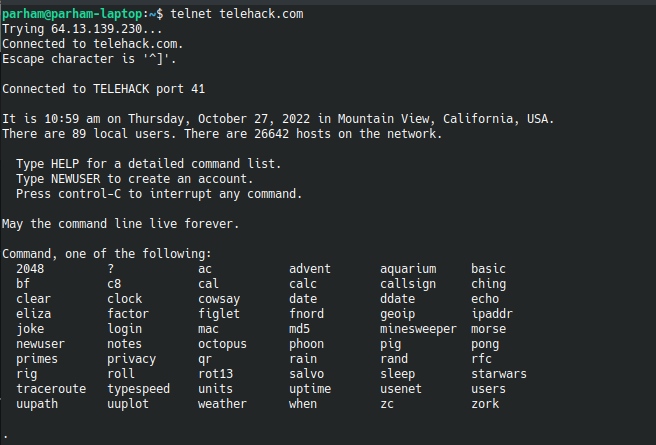
\includegraphics[width=0.9\textwidth]{src/teleinit.png}
	\caption{
		ورودی telnet
	}
	\label{fig:telinit}
\end{figure}
\begin{figure}[h!]
	\centering
	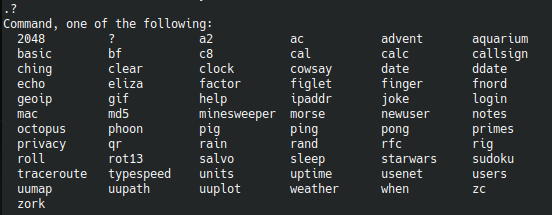
\includegraphics[width=0.9\textwidth]{src/telhelp.png}
	\caption{
		خروجی دستور $?$
	}
	\label{fig:telhelp}
\end{figure}
\begin{figure}[h!]
	\centering
	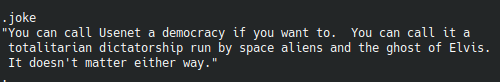
\includegraphics[width=0.9\textwidth]{src/teljoke.png}
	\caption{
		خروجی دستور joke
	}
	\label{fig:teljoke}
\end{figure}
\begin{figure}[h!]
	\centering
	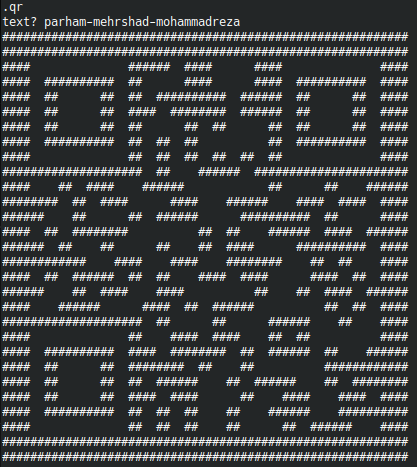
\includegraphics[width=0.9\textwidth]{src/telqr.png}
	\caption{
		خروجی دستور telqr با استفاده از متن parham-mehrshad-mohammadreza
	}
	\label{fig:telqr}
\end{figure}
\begin{figure}[h!]
	\centering
	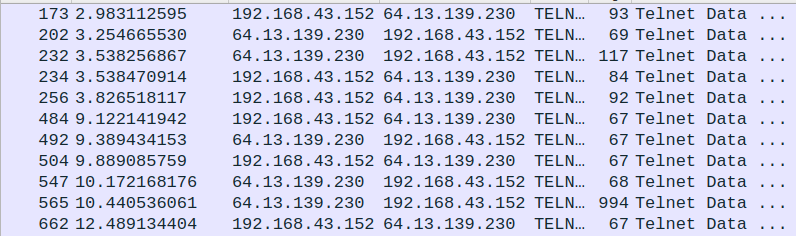
\includegraphics[width=0.9\textwidth]{src/telwire.png}
	\caption{
		داده‌های telnet در wireshark
	}
	\label{fig:telnetwire}
\end{figure}
\begin{figure}[h!]
	\centering
	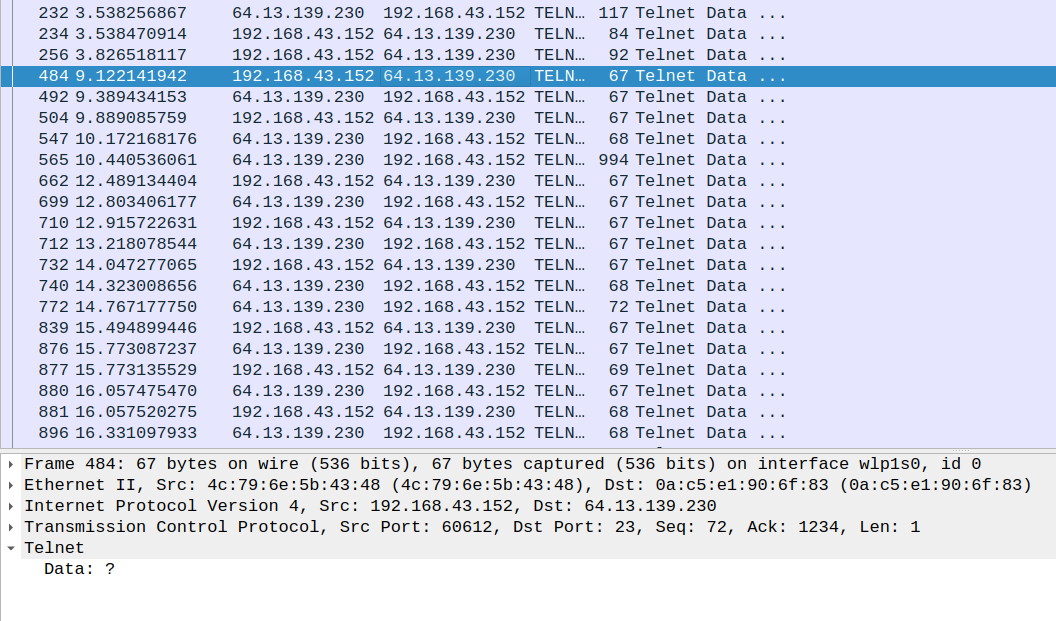
\includegraphics[width=0.9\textwidth]{src/telnetcharsend.png}
	\caption{
		کاراکتر ارسالی
	}
	\label{fig:telnetcharsend}
\end{figure}
\begin{figure}[h!]
	\centering
	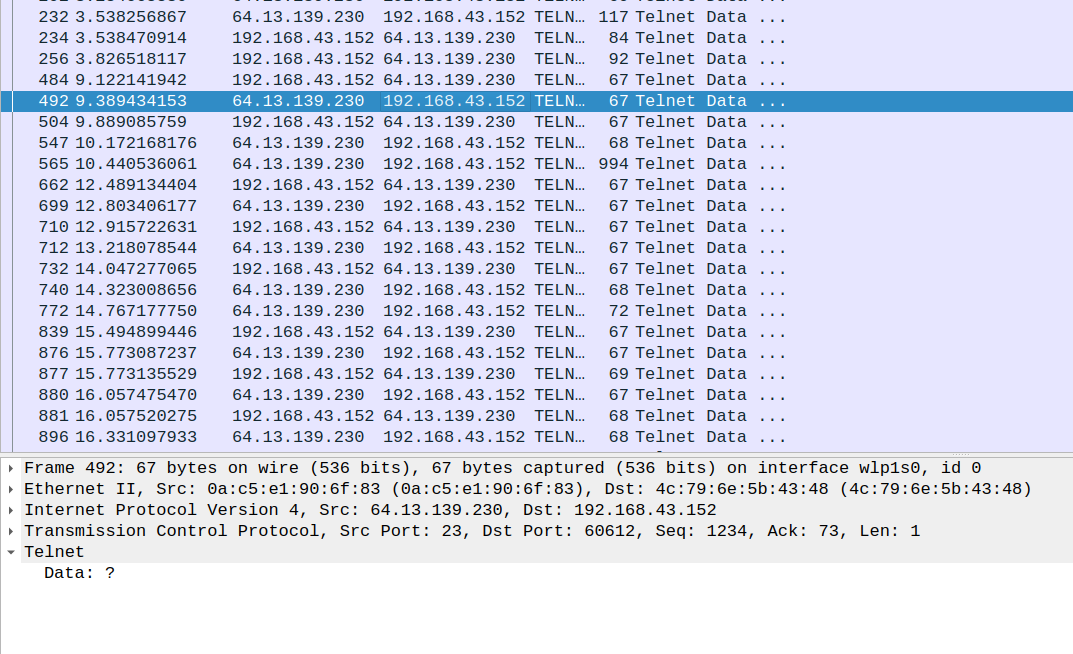
\includegraphics[width=0.9\textwidth]{src/telnetcharrec.png}
	\caption{
		کاراکتر دریافتی
	}
	\label{fig:telnetcharrec}
\end{figure}
\begin{figure}[h!]
	\centering
	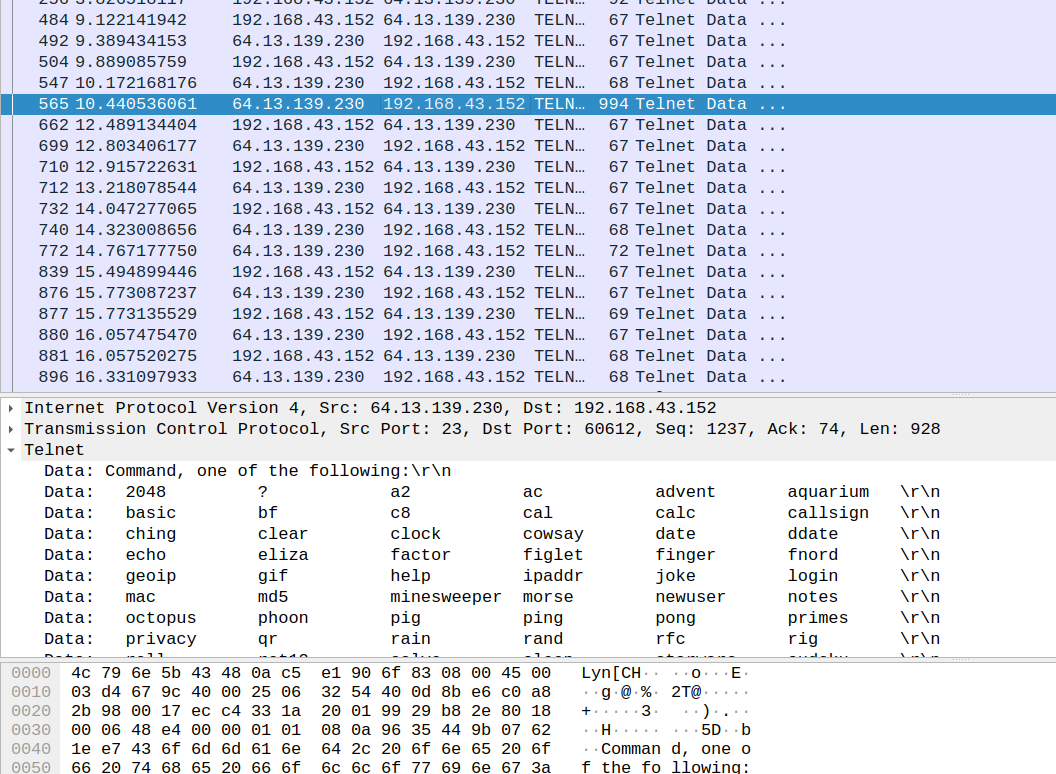
\includegraphics[width=0.9\textwidth]{src/telhelpcharresp.png}
	\caption{
		جواب دریافتی
	}
	\label{fig:telhelpcharresp}
\end{figure}
\subsection{سوال اول}
با باز کردن داده‌های گفته شده با تصویر \ref{fig:teldata} مواجه می‌شویم. با توجه داده‌ها متوجه می‌شویم که آدرس مبدا برابر با 
2.0.168.192 
و آدرس مقصد برابر با
1.0.168.192 
می‌باشد.
\begin{figure}[h!]
	\centering
	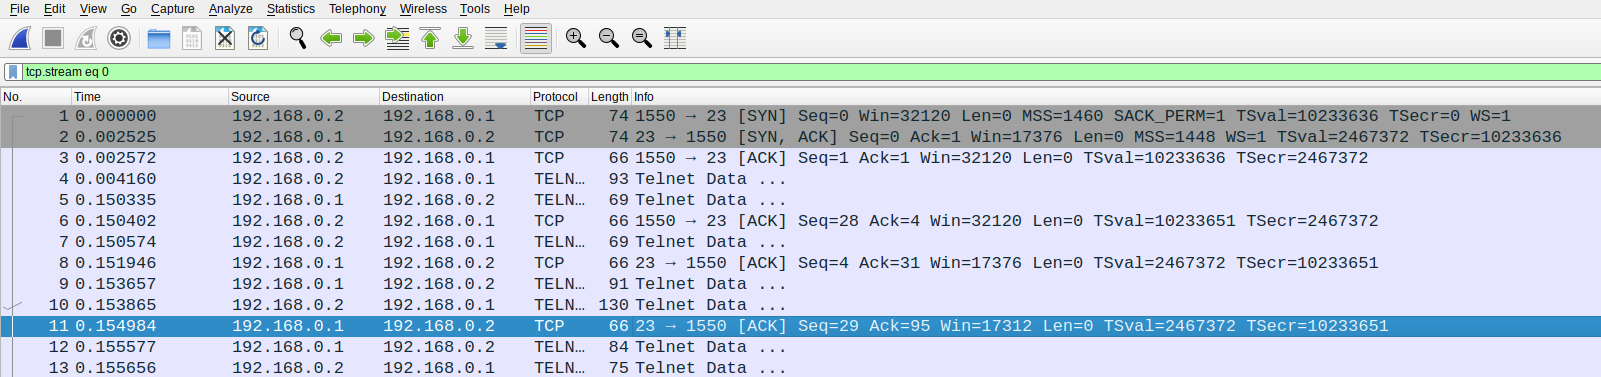
\includegraphics[width=0.9\textwidth]{src/teldata.png}
	\caption{
		داده‌های مشاهده شده در فایل telnet.pcap
	}
	\label{fig:teldata}
\end{figure}
\subsection{سوال دوم}
با راست کلیک روی بسته‌ی اول، زدن follow و 
\lr{TCP Stream} 
می‌توانیم روند طی شده را مشاهده کنیم. خروجی در شکل \ref{fig:teldetail} مشاهده می‌شود. می‌توان متوجه شد که یوزرنیم کاربر برابر با fake بوده و رمز عبور وی برابر با user بوده است.
\begin{figure}[h!]
	\centering
	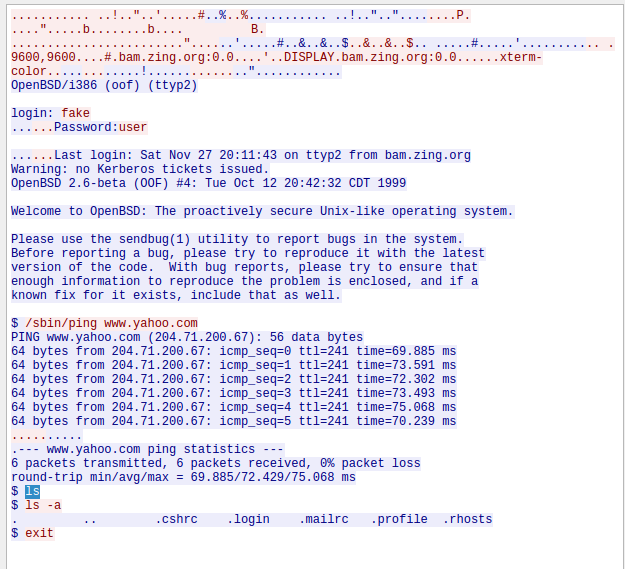
\includegraphics[width=0.9\textwidth]{src/teldetail.png}
	\caption{
		داده‌های وارد شده و دریافت شده توسط کاربر
	}
	\label{fig:teldetail}
\end{figure}
\subsection{سوال سوم}
دوباره با مراجعه به شکل  \ref{fig:teldetail}، می‌توان متوجه شد که دستور‌های زده شده به ترتیب به صورت زیر می‌باشند: (بین دستور اول و دوم هم interrupt فرستاده است تا فرایند ping قطع شود)
\begin{flushleft}
	\lr{\lr{/sbin/ping www.yahoo.com}, ls, \lr{ls -a}, exit}
\end{flushleft}
\section{بخش سوم}
ما سایت github.com را انتخاب کردیم. در شکل \ref{fig:digout} می‌توان خروجی‌های مربوط به این دستور را در wireshark مشاهده کرد. شکل \ref{fig:flagsquery} شامل flagهای دستور dns برای پکت ارسالی می‌باشد و شکل \ref{fig:flagsresp} شامل flagهای دستور dns برای پکت دریافتی می‌باشد. همچنین در شکل \ref{fig:digrunterm} می‌توانید نتیجه‌ی اجرای دستور dig در ترمینال را مشاهده کنید.
\begin{figure}[h!]
	\centering
	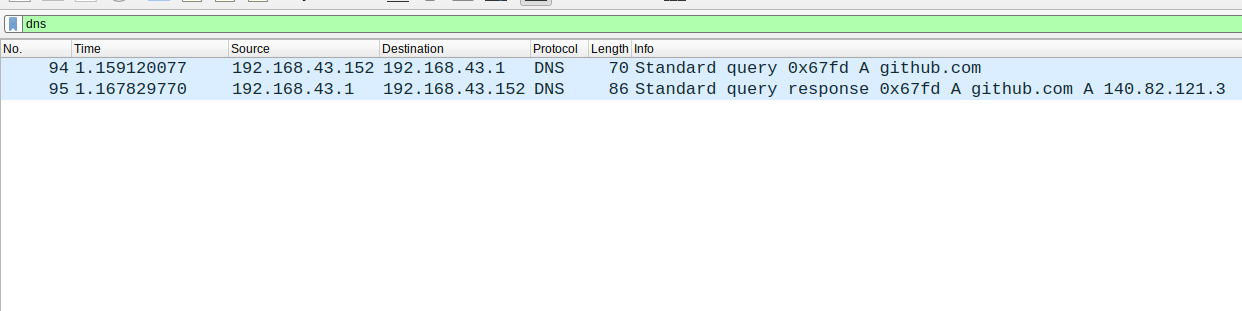
\includegraphics[width=0.9\textwidth]{src/digrun.png}
	\caption{
		خروجی‌های دستور dig در نرم‌افزار wireshark
	}
	\label{fig:digout}
\end{figure}
\begin{figure}[h!]
	\centering
	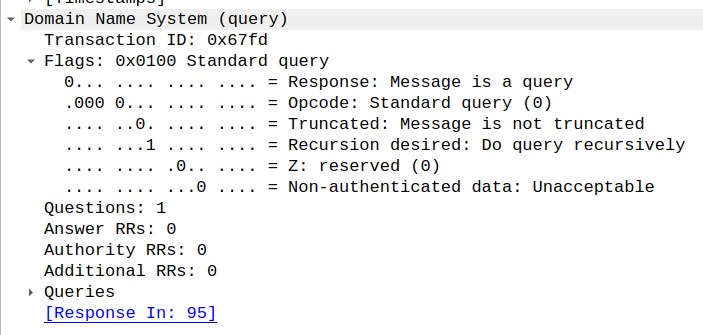
\includegraphics[width=0.9\textwidth]{src/flagsquery.png}
	\caption{
		پرچم‌های سوال dns در wireshark
	}
	\label{fig:flagsquery}
\end{figure}
\begin{figure}[h!]
	\centering
	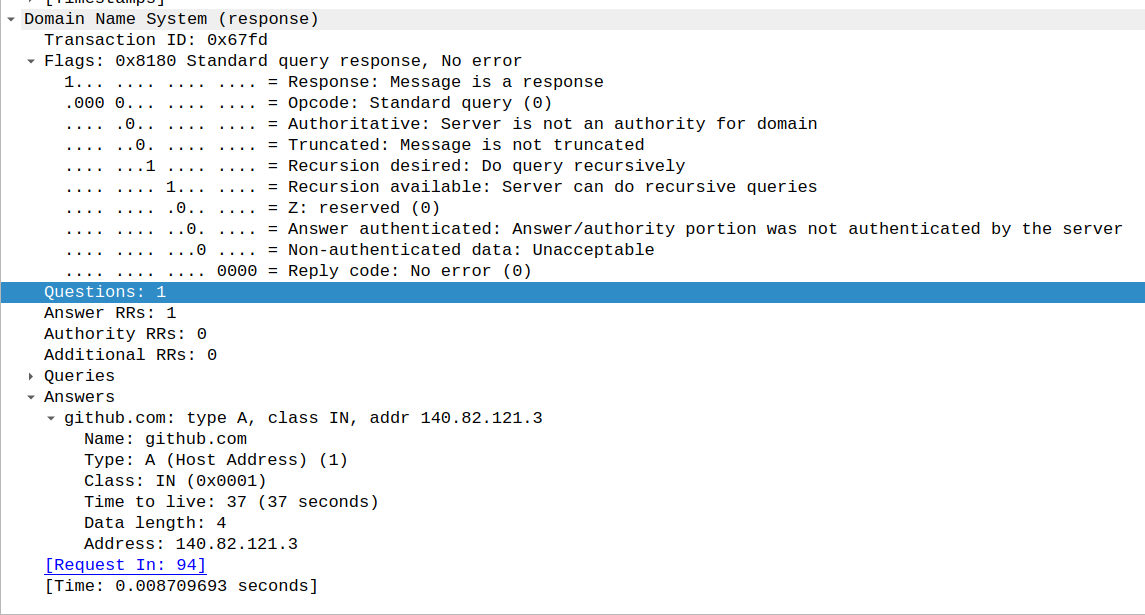
\includegraphics[width=0.9\textwidth]{src/flagsresp.png}
	\caption{
		پرچم‌های mhso dns در wireshark
	}
	\label{fig:flagsresp}
\end{figure}
\begin{figure}[h!]
	\centering
	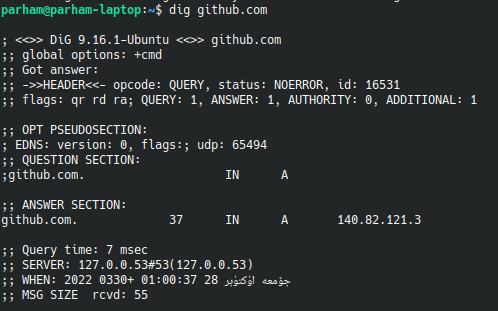
\includegraphics[width=0.9\textwidth]{src/digrunterm.png}
	\caption{
		خروجی دستور dig در ترمینال
	}
	\label{fig:digrunterm}
\end{figure}
\subsection{سوال اول}
همانطور که در شکل \ref{fig:digout} مشاهده می‌شود، این درخواست برای سرور 1.43.168.192 ارسال می‌شود و جواب نیز از آن دریافت می‌شود. علت این است که در تنظیمات مربوط به کامپیوتر این سرور لوکال برای dns ذخیره شده است.
\subsection{سوال دوم}
این سوال را با توجه به شکل‌های \ref{fig:flagsquery} و \ref{fig:flagsresp} پاسخ می‌دهیم. ابتدا لازم به ذکر است که هدر‌های یک پیام dns شامل بخش‌های مختلقی است این بخش‌ها عبارتند از: 
\lr{Trunction ID}, 
\lr{Flags}, 
Questions,
\lr{Answer RRs},
\lr{Authority RRs},
\lr{Additional RRs},
\lr{Queries} 
که حال به بررسی آن‌ها می‌پردازیم. مورد اول که TID می‌باشد شماره‌ی مخصوصی است که مشخص می‌کند یک جواب مربوط به چه سوالی است. پرچم‌ها را در انتها بررسی می‌کنیم. قسمت بعدی سوال‌هاست که اینجا عدد آن برابر یک است. قسمت بعدی جواب‌هاست که برای کوئری این عدد برابر ۰ است و برای پاسخ این عدد برابر با ۱ است.

قسمت Authority و Additional برای هر دو یکسان است. در قسمت Queries که این هم یکسان است درخواست ارسالی به سرور را مشاهده می‌کنیم که گیتهاب است. برای پاسخ قسمت Answers نیز داریم که جواب دریافت شده از سرور را نشان می‌دهد، اطلاعات مهمی که در آن حاضر است عبارت است از زمان اعتبار داشتن جواب، آی‌پی، و نام می‌باشد.

پرچم‌ها نیز قسمت‌های یکسان زیادی دارند ابتدا آن‌ها را نام می‌بریم و توضیح می‌دهیم. اولین پرچم مشخص می‌کند که این پکت query است یا answer. در ادامه trunctated نشان می‌دهد که بسته کامل است یا نه که در این مثال هر دو بسته کامل می‌باشند. recursion مشخص می‌کند که آیا سرور باید درخواست را به سرور‌های دیگر بفرستد یا نه که برای پاسخ و جواب \lr{recursion desired} داریم که نشان می‌دهد آیا سرور مجاز به این کار است یا نه. در پاسخ یک پرچم اضافی در این مورد داریم به نام 
\lr{recursion available } 
که نشان می‌دهد آیا سرور توانایی این کار را دارد یا نه.

پرچم دیگری که در هر دو یکسان  است non-authenticated-date است که نشان می‌دهد آیا پاسخ authenticate نشده قابل قبول است یا نه که در این مثال برای هر دو غیر قابل قبول مشخص شده.

در نهایت replay-code مشخص می‌کند که وضعیت پاسخ به چه گونه است. در این مثال خطایی وجود نداشته و وضعیت با ۰ گزارش شده است.
\end{document}
